\documentclass[12pt]{article}

\usepackage{fancyhdr} % Required for custom headers
\usepackage{lastpage} % Required to determine the last page for the footer
\usepackage{extramarks} % Required for headers and footers
\usepackage[usenames,dvipsnames]{color} % Required for custom colors
\usepackage{graphicx} % Required to insert images
\usepackage{listings} % Required for insertion of code
\usepackage{courier} % Required for the courier font
\usepackage{lipsum} % Used for inserting dummy 'Lorem ipsum' text into the template
\usepackage{amsmath}
\usepackage{caption}
\usepackage[dvipsnames]{xcolor}

% Margins
\topmargin=-0.45in
\evensidemargin=0in
\oddsidemargin=0in
\textwidth=6.5in
\textheight=9.0in
\headsep=0.25in
\headheight=15.0pt


\linespread{1.1} % Line spacing

% Set up the header and footer
\pagestyle{fancy}
\lhead{\hmwkAuthorName} % Top left header
\chead{\hmwkClass: \hmwkTitle} % Top center head
\cfoot{} % Bottom center footer
\rfoot{Page\ \thepage\ of\ \protect\pageref{LastPage}} % Bottom right footer
\renewcommand\headrulewidth{0.4pt} % Size of the header rule
\renewcommand\footrulewidth{0.4pt} % Size of the footer rule

\setlength\parindent{0pt} % Removes all indentation from paragraphs

%----------------------------------------------------------------------------------------
%	DOCUMENT STRUCTURE COMMANDS
%	Skip this unless you know what you're doing
%----------------------------------------------------------------------------------------

% Header and footer for when a page split occurs within a problem environment
\newcommand{\enterProblemHeader}[1]{
	\nobreak\extramarks{#1}{#1 continued on next page\ldots}\nobreak
	\nobreak\extramarks{#1 (continued)}{#1 continued on next page\ldots}\nobreak
}

% Header and footer for when a page split occurs between problem environments
\newcommand{\exitProblemHeader}[1]{
	\nobreak\extramarks{#1 (continued)}{#1 continued on next page\ldots}\nobreak
	\nobreak\extramarks{#1}{}\nobreak
}

\setcounter{secnumdepth}{0} % Removes default section numbers
\newcounter{homeworkProblemCounter} % Creates a counter to keep track of the number of problems

\newcommand{\homeworkProblemName}{}
\newenvironment{homeworkProblem}[1][Problem \arabic{homeworkProblemCounter}]{ % Makes a new environment called homeworkProblem which takes 1 argument (custom name) but the default is "Problem #"
	\stepcounter{homeworkProblemCounter} % Increase counter for number of problems
	\renewcommand{\homeworkProblemName}{#1} % Assign \homeworkProblemName the name of the problem
	\section{\homeworkProblemName} % Make a section in the document with the custom problem count
	\enterProblemHeader{\homeworkProblemName} % Header and footer within the environment
}{
	\exitProblemHeader{\homeworkProblemName} % Header and footer after the environment
}

\newcommand{\problemAnswer}[1]{ % Defines the problem answer command with the content as the only argument
	\noindent\framebox[\columnwidth][c]{\begin{minipage}{0.98\columnwidth}#1\end{minipage}} % Makes the box around the problem answer and puts the content inside
}

\newcommand{\homeworkSectionName}{}
\newenvironment{homeworkSection}[1]{ % New environment for sections within homework problems, takes 1 argument - the name of the section
	\renewcommand{\homeworkSectionName}{#1} % Assign \homeworkSectionName to the name of the section from the environment argument
	\subsection{\homeworkSectionName} % Make a subsection with the custom name of the subsection
	\enterProblemHeader{\homeworkProblemName\ [\homeworkSectionName]} % Header and footer within the environment
}{
	\enterProblemHeader{\homeworkProblemName} % Header and footer after the environment
}

%----------------------------------------------------------------------------------------
%	NAME AND CLASS SECTION
%----------------------------------------------------------------------------------------

\newcommand{\hmwkTitle}{Assignment\ \#1} % Assignment title
\newcommand{\hmwkClass}{Advanced Image Processing} % Course/class
\newcommand{\hmwkClassInstructor}{Jones} % Teacher/lecturer
\newcommand{\hmwkAuthorName}{Shikhar Vashishth} % Your name
\newcommand{\hmwkAuthorID}{M.Tech CSA - 13374} % Your ID

%----------------------------------------------------------------------------------------
%	TITLE PAGE
%----------------------------------------------------------------------------------------

\title{
	\vspace{2in}
	\textmd{\textbf{\hmwkClass}}\\ 
	\textmd{\textbf{\hmwkTitle}}\\
	\vspace{3in}
}

\author{\textbf{\hmwkAuthorName} \\ {\small \hmwkAuthorID}}
\date{} % Insert date here if you want it to appear below your name

%----------------------------------------------------------------------------------------

\begin{document}
	
\maketitle
\newpage

\begin{homeworkProblem}
	

\subsubsection*{Implementation:}

\paragraph{Gradient Based:}
Sobel filter, a gradient-based edge detector, has been used for detecting edges in the image. For implementing this method two sobel operators were created of 3x3 size for calculating gradient along horizontal and vertical directions. 

\[
S_x=
\begin{bmatrix}
-1 & 0 & 1 \\
-2 & 0 & 2 \\
-1 & 0 & 1 
\end{bmatrix}
\]

\[
S_y=
\begin{bmatrix}
 1 & 2 & 1 \\
 0 & 0 & 0 \\
-1 & -2 &-1 
\end{bmatrix}
\]

These operators were convolved with the image to give gradients along x and y directions as $I_x$ and $I_y$. Finally, gradient magnitude was calculated as and a threshold was chosen to get the edges
$$ G = \sqrt{{I_x}^2 + {I_y}^2}$$

\paragraph{Laplacian of Gaussian} For implementing LOG method, directly LOG filter of size (9x9) was computed using the following formula and with sigma value as 1.0. Then the filter was convolved with the image and based on the image a threshold was guessed to get the edges.
$$ - \frac{1}{\pi \sigma^4} \left[1 - \frac{(x^2+y^2)}{2\sigma^2} \right] e^{-\frac{(x^2+y^2)}{2\sigma^2}} $$

\paragraph{Noise} For comparing the performance of the gradient-based and LOG algorithm at different level of noise, I have introduced Gaussian noise in the original image with mean zero and variable variance. Level of noise was increased by increasing the value of variance(sigma). A matrix of the size of image filled with normally distributed random numbers was created using 'randn' function provided by OpenCV and was added to the original image. 

\paragraph{Selecting Threshold value}
For selecting an appropriate value of threshold, a number of threshold values were used and the one giving visually the best result was chosen. The following figures shows the outcome on using different thresholds for both the methods. The guesses for threshold values were made based on the range of values For gradient-based method the best output came at threshold value 300 whereas for the LOG method the best result came at around 17.5.
$$ \text{Final output} =  \text{Image} > threshold$$

\begin{figure}[ht]
	\centering
	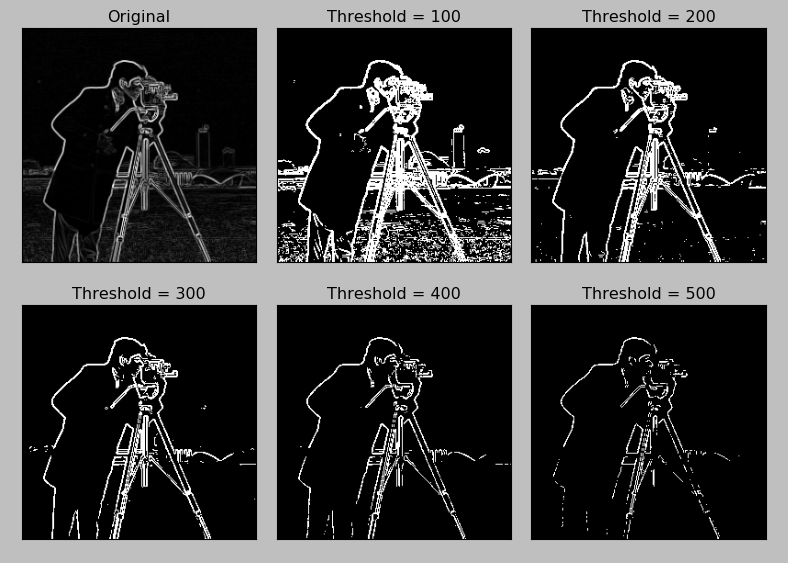
\includegraphics[width=14cm]{/home/shikhar/Documents/PycharmProjects/Assignment-1/Solution_Report/q1/thresh_grad.png}
	\caption{Selecting threshold for gradient based method}
\end{figure}

\begin{figure}[ht]
	\centering
	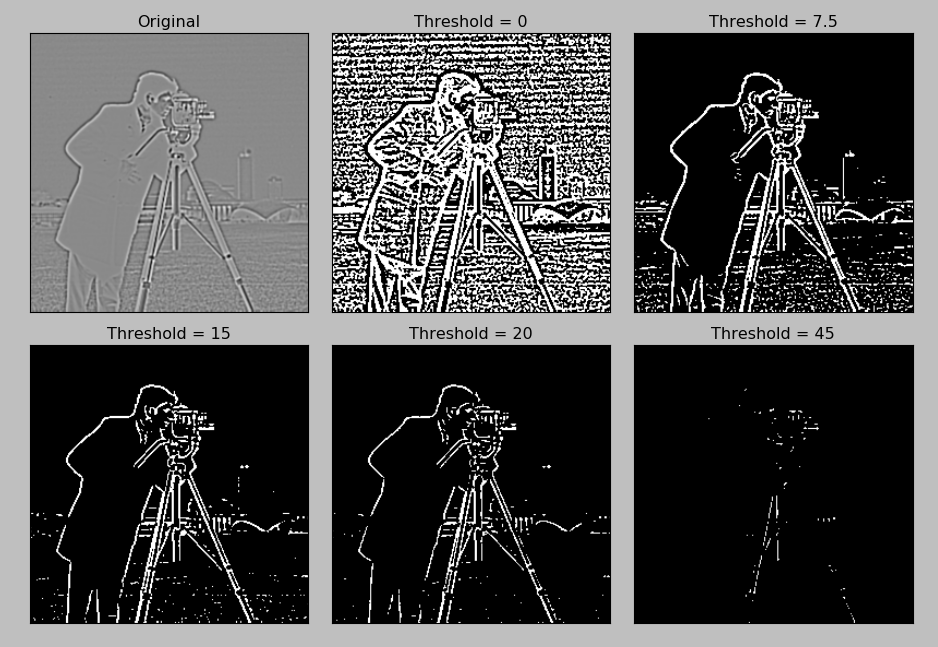
\includegraphics[width=14cm]{/home/shikhar/Documents/PycharmProjects/Assignment-1/Solution_Report/q1/thresh_log.png}
	\caption{Selecting threshold for LOG method}
\end{figure}

\clearpage
\subsubsection*{Results:}
\paragraph{}
The following figures shows the performance of these two methods on an image with different noise levels. The observations from the results are:
\begin{enumerate}
	\item LOG method is capable of detecting fine edges as compared to gradient-based methods because it is based on calculating 2nd derivative. But that makes it more susceptible to noise in the image as can be seen from the results. At sigma value 16.0 we can clearly see that LOG results has got corrupted by noise whereas the Sobel result is much more better.
	\item On the other hand, the gradient based method although is more robust to noise than LOG but produces thicker edges and misses out finer edges in the image.
	\item Since, Sobel method was used for edge detection therefore, the diagonal edges detected are much more thicker than the horizontal and vertical edges because gradient magnitude is calculated as  $\sqrt{{I_x}^2 + {I_y}^2}$

\end{enumerate}

\begin{figure}[ht]
	\centering
	\caption*{\textbf{Comparing Gradient-based and LOG method for different noise levels}}
	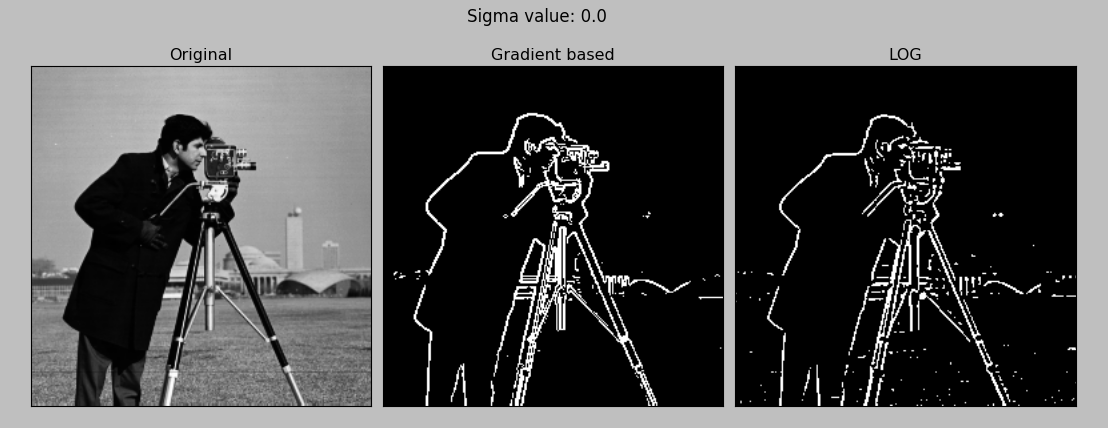
\includegraphics[width=16cm]{/home/shikhar/Documents/PycharmProjects/Assignment-1/Solution_Report/q1/noise_1.png}
	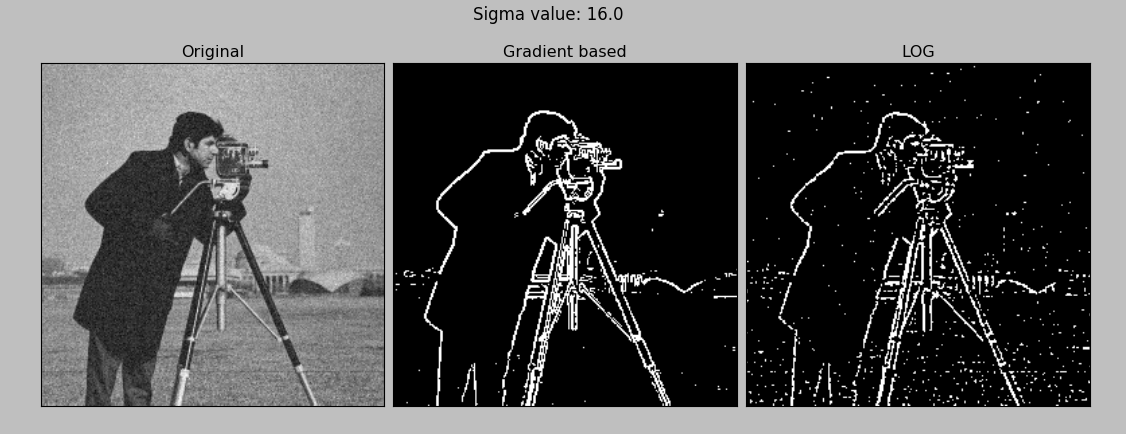
\includegraphics[width=16cm]{/home/shikhar/Documents/PycharmProjects/Assignment-1/Solution_Report/q1/noise_2.png}
	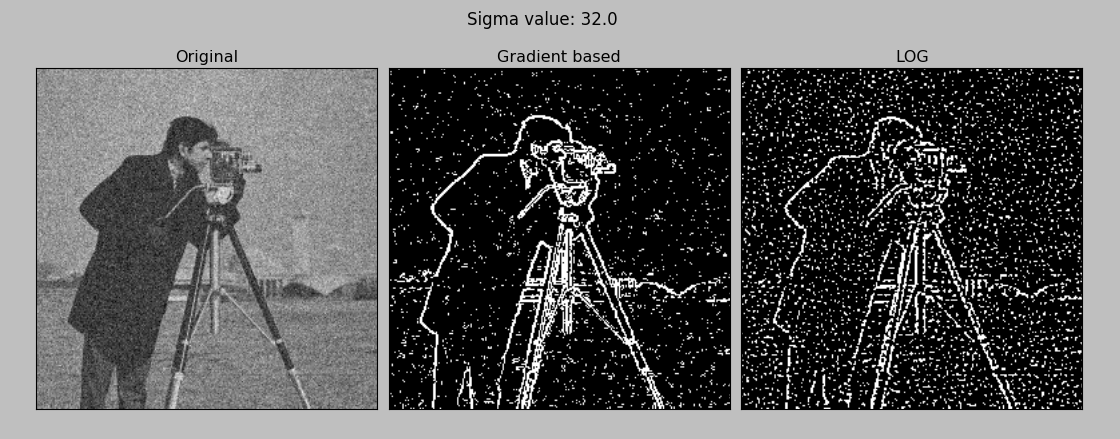
\includegraphics[width=16cm]{/home/shikhar/Documents/PycharmProjects/Assignment-1/Solution_Report/q1/noise_3.png}
\end{figure}

\begin{figure}[ht]
	\centering
	\caption*{\textbf{Comparing Gradient-based and LOG method for different noise levels}}
	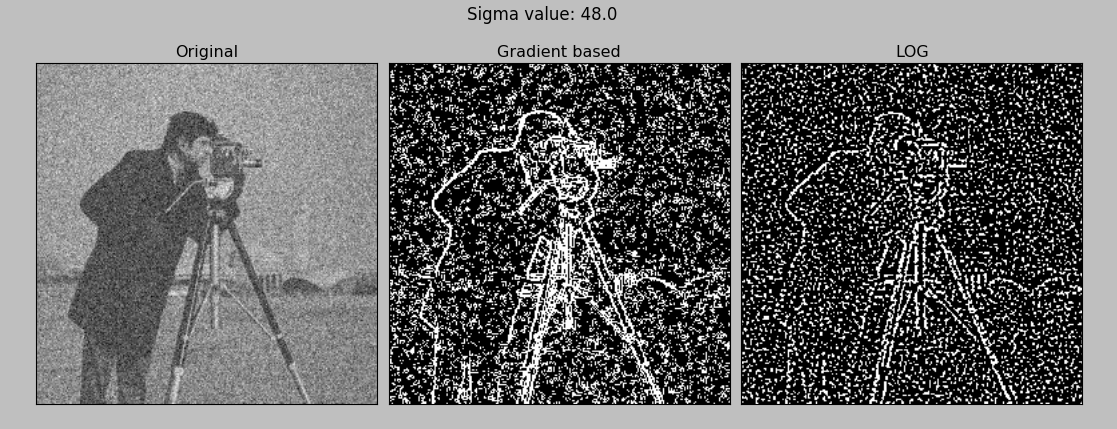
\includegraphics[width=16cm]{/home/shikhar/Documents/PycharmProjects/Assignment-1/Solution_Report/q1/noise_4.png}
	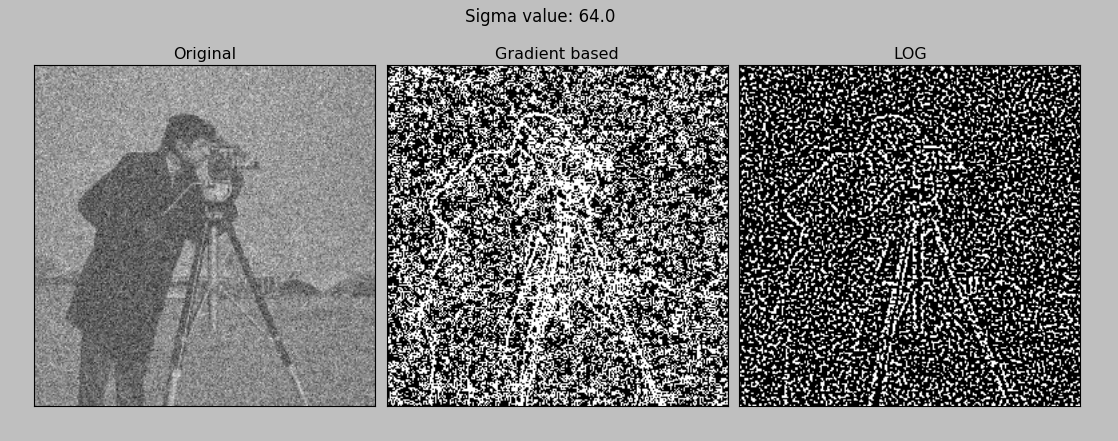
\includegraphics[width=16cm]{/home/shikhar/Documents/PycharmProjects/Assignment-1/Solution_Report/q1/noise_5.png}
	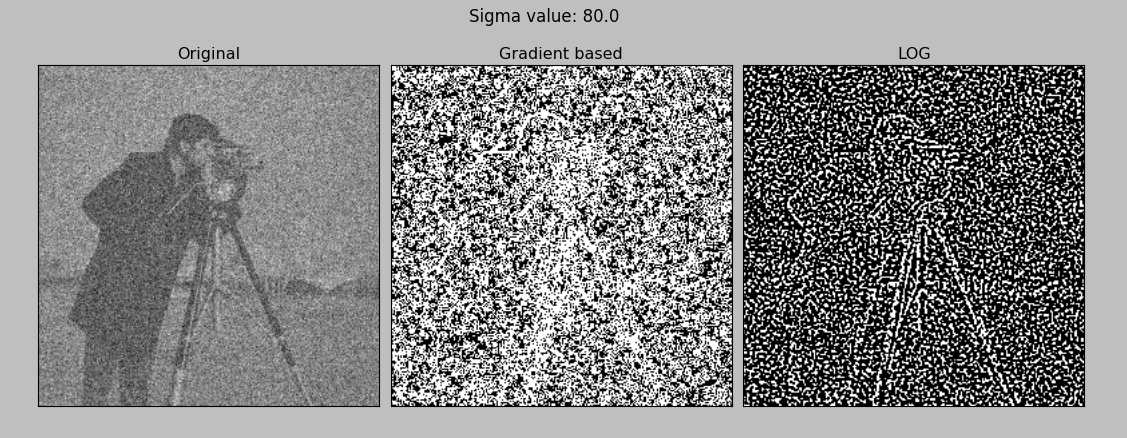
\includegraphics[width=16cm]{/home/shikhar/Documents/PycharmProjects/Assignment-1/Solution_Report/q1/noise_6.png}
\end{figure}

\end{homeworkProblem}

\clearpage
\begin{homeworkProblem}

\subsection*{Implementation}
\paragraph{}
I have used the standard implementation of the SIFT algorithm which comes with OpenCV library (opencv\_contrib). For matching two images, I first computed the desciptors of both the images and then for each descriptor I find out its two best matches using k-nearest neighbor algorithm with k=2 so that ratio test as described by D.Lowe in his SIFT paper could be used. A match is accepted if:
$$\frac{SSD(f_1,f_2)}{SSD(f_1,f_2')}  \le 0.8$$

\subsubsection{Affine transformation}
\paragraph{}
The original image was transformed using a affine transformation. For the transformation the following matrix was used which scales the image by a factor of 1.2 and rotates it counter-clockwise by 30$^{\circ}$.
\[
M=
\begin{bmatrix}
1.2*\cos{30^{\circ}} & \sin{30^{\circ}} & 0 \\
\sin{30^{\circ}} & 1.2*\cos{30^{\circ}} & 0 
\end{bmatrix}
\]

\subsubsection{Noise}
\paragraph{}
The salt-pepper noise was introduced in the image by blending it with a random matrix of the dimensions same as that of the image and with entries uniformly distributed between 0 and 255.
$$Noise = rand(dims, 0 , 255)$$
$$Img = \alpha * Img + (1 - \alpha) Noise \text{  ; $\alpha = 0.2$}$$

\subsubsection{Changing illumination}
\paragraph{}
For changing the illumination of the image a constant was added to it and the pixel intensities which exceeded 255 were set to 255.

\clearpage
\subsection*{Results:}
\paragraph{}
The figure below shows the detected keypoints in the original and the transformed images using SIFT algorithm. The circles for the keypoints are drawn according to their size and along with their orientation. The number in the bracket shows the number of the keypoints in the image. 

\subsubsection{Observations:}
\begin{enumerate}
	\item The number of keypoints in the image increased as we introduced noise in the image because noise creates finer details which get detected as keypoints by the algorithm
	\item Affine and occlusion transform reduced the number of keypoints because the part of the image got removed because of scaling, rotation and cropping.
	\item The flipped image has almost the same number of descriptors as the original image but the orientation of all descriptors has also got flipped.
	\item Image with changed illumination has less number of keypoints because some of details of image got lost because of the saturation of pixel intensity values.
	
\end{enumerate}

\clearpage
\begin{center}
	\begin{tabular}{||c c c c||} 
		\hline
		\textbf{Image index} & \textbf{Transf Type} & \textbf{\# of Descriptors} & \textbf{Change in Descriptors}\\ [0.5ex] 
		\hline\hline
		(0,0) & Original 			& 145 & 0\% \\ \hline
		(0,1) & Noise 				& 344 & +137\% \\ \hline
		(1,0) & Affine \& Occlusion & 141 & -2.75\% \\ \hline
		(1,1) & Noise \& Affine 	& 515 & +255.17\% \\ \hline
		(2,0) & Illumination 		& 65 & -55.17\% \\ \hline
		(2,1) & Flip 				& 144 & -0.68\% \\ \hline
	\end{tabular}
\end{center}

\begin{figure}[h]
	\centering
	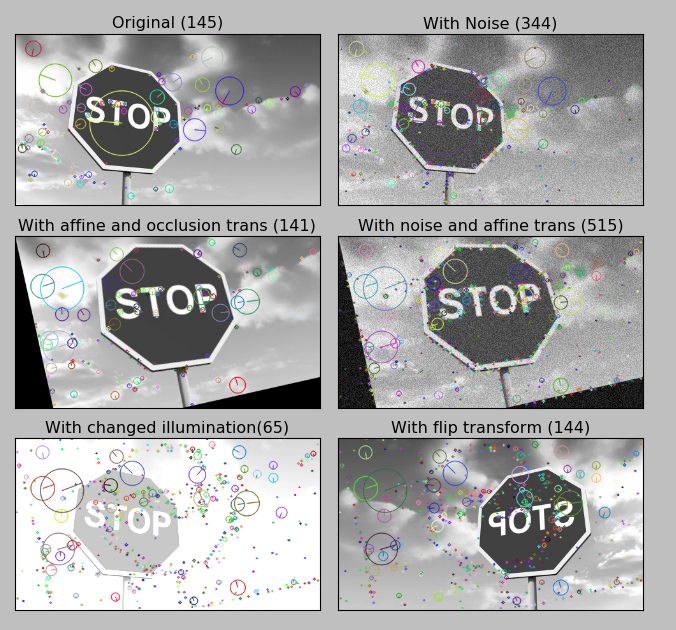
\includegraphics[width=14cm]{/home/shikhar/Documents/PycharmProjects/Assignment-1/Solution_Report/q2/img_kp2.png}
	\caption{Showing Keypoints with their size and orientation}
\end{figure}

\clearpage
\begin{center}
	\begin{tabular}{||c c c c||} 
		\hline
		\textbf{Image index} & \textbf{Transf Type} & \textbf{\# of Descriptors} & \textbf{Change in Descriptors}\\ [0.5ex] 
		\hline\hline
		(0,0) & Original 			& 206 & 0\% \\ \hline
		(0,1) & Noise 				& 292 & +41.74\% \\ \hline
		(0,2) & Affine \& Occlusion & 143 & -30.58\% \\ \hline
		(1,0) & Noise \& Affine 	& 289 & +40.29\% \\ \hline
		(1,1) & Illumination 		& 65 & -68.44\% \\ \hline
		(2,2) & Flip 				& 213 & +3.34\% \\ \hline
	\end{tabular}
\end{center}

\begin{figure}[h]
	
	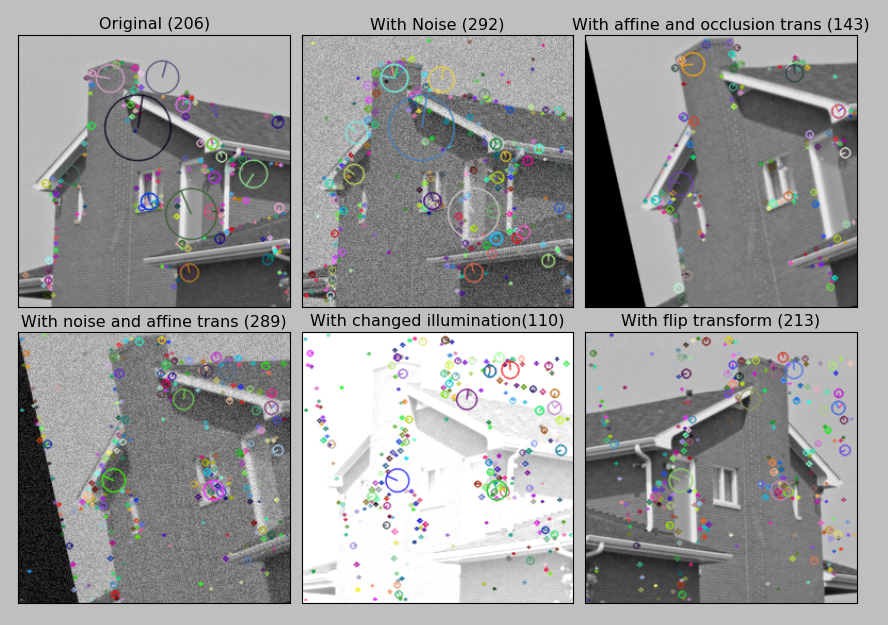
\includegraphics[width=16cm]{/home/shikhar/Documents/PycharmProjects/Assignment-1/Solution_Report/q2/img_kp1.png}
	\caption{Showing Keypoints with their size and orientation}
	\centering
\end{figure}



\clearpage
\paragraph{Matching}
The matching was done using k-nearest neighbor approach. The observations are as follows:
\begin{enumerate}
	\item The first result, verifies the scale and rotational invariant nature of the SIFT algorithm which is the most important advantage with SIFT.
	\item The algorithm performs well even in the presence of noise
	\item The algorithm gave around 25\% match when illumination of the image is changed. It shows that it is not invariant to change in illumination.
	\item The algorithm performs poorly when comparing with flipped image which shows  that although it is invariant to rotation but couldn't perform well when image is flipped.
\end{enumerate}

\begin{center}
	\begin{tabular}{||c c c||} 
		\hline
		\textbf{Trans Type} & \textbf{\# of Matched Descriptors} & \textbf{\% of matched Descriptors}\\ [0.5ex] 
		\hline\hline
		Affine \& Occlusion 	& 75 & 52.08\% \\ \hline
		Noise 			& 79 & 54.48\% \\ \hline
		Noise \& Affine 	& 60 & 41.37\% \\ \hline
		Illumination 		& 35 & 24.13\% \\ \hline
		Flip 			& 39 & 26.89\% \\ \hline
	\end{tabular}
\end{center}

\begin{figure}[h]
	\centering
	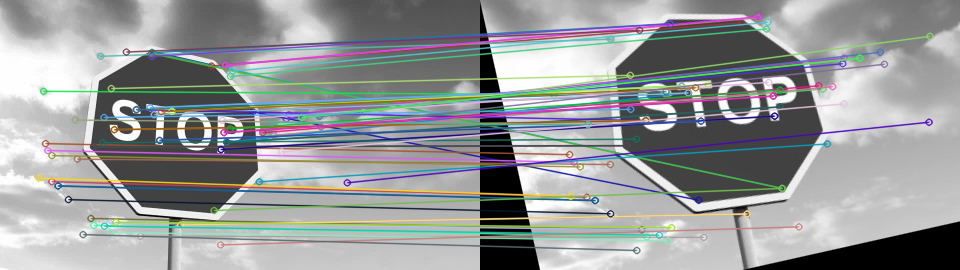
\includegraphics[scale=.4]{/home/shikhar/Documents/PycharmProjects/Assignment-1/Solution_Report/q2/match2_1.png}
	\caption{Matching with Affine transformed image}
\end{figure}
\begin{figure}[h]
	\centering
	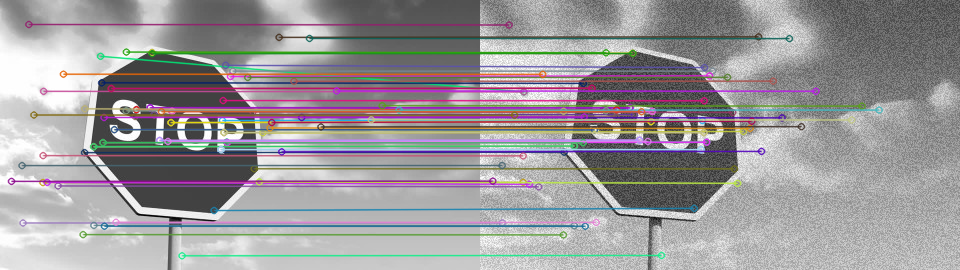
\includegraphics[scale=.4]{/home/shikhar/Documents/PycharmProjects/Assignment-1/Solution_Report/q2/match2_2.png}
	\caption{Matching with noisy image}
\end{figure}
\begin{figure}[h]
	\centering
	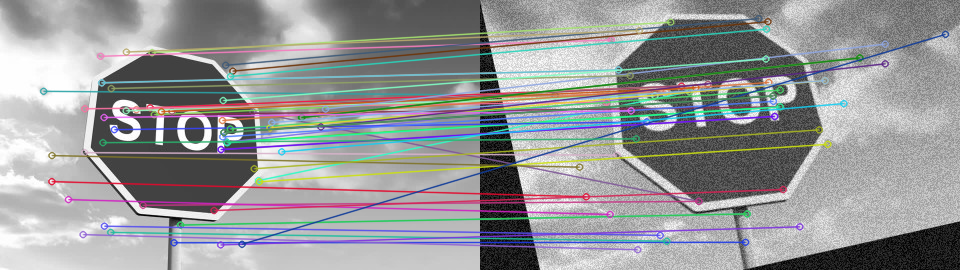
\includegraphics[scale=.4]{/home/shikhar/Documents/PycharmProjects/Assignment-1/Solution_Report/q2/match2_3.png}
	\caption{Matching with affine transformed and noisy image}
\end{figure}
\begin{figure}[h]
	\centering
	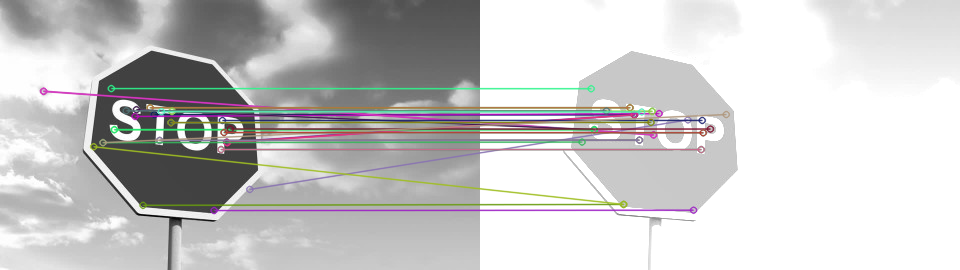
\includegraphics[scale=.4]{/home/shikhar/Documents/PycharmProjects/Assignment-1/Solution_Report/q2/match2_4.png}
	\caption{Matching with changed illumination }
\end{figure}
\begin{figure}[h]
	\centering
	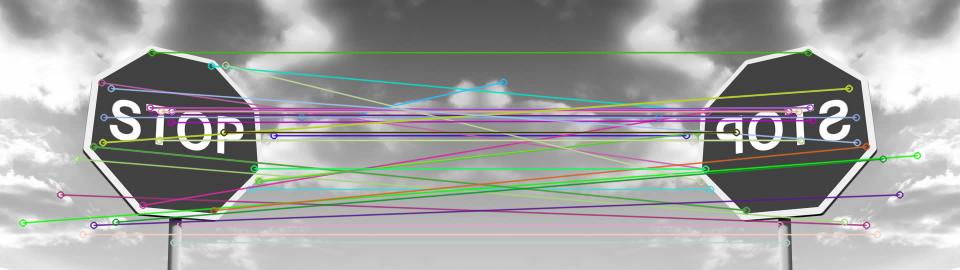
\includegraphics[scale=.4]{/home/shikhar/Documents/PycharmProjects/Assignment-1/Solution_Report/q2/match2_5.png}
	\caption{Matching with flipped image}
\end{figure}

\clearpage
\begin{center}
	\begin{tabular}{||c c c||} 
		\hline
		\textbf{Trans Type} & \textbf{\# of Matched Descriptors} & \textbf{\% of matched Descriptors}\\ [0.5ex] 
		\hline\hline
		Affine \& Occlusion 	& 90 & 43.68\% \\ \hline
		Noise 			& 95 & 46.11\% \\ \hline
		Noise \& Affine 	& 76 & 36.89\% \\ \hline
		Illumination 		& 54 & 26.21\% \\ \hline
		Flip 			& 52 & 25.24\% \\ \hline
	\end{tabular}
\end{center}

\begin{figure}[h]
	\centering
	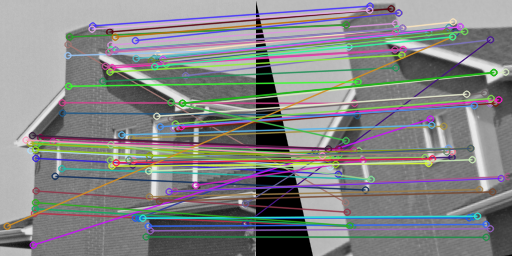
\includegraphics[scale=0.6]{/home/shikhar/Documents/PycharmProjects/Assignment-1/Solution_Report/q2/match1_1.png}
	\caption{Matching with Affine transformed image}
\end{figure}
\begin{figure}[h]
	\centering
	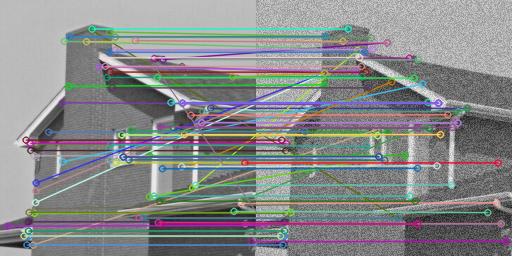
\includegraphics[scale=0.6]{/home/shikhar/Documents/PycharmProjects/Assignment-1/Solution_Report/q2/match1_2.png}
	\caption{Matching with noisy image}
\end{figure}
\begin{figure}[h]
	\centering
	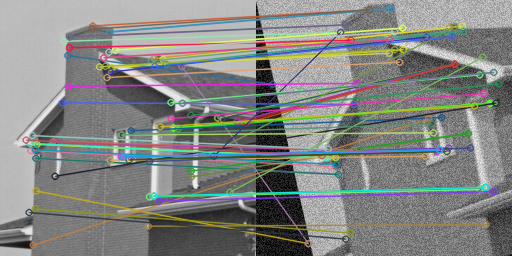
\includegraphics[scale=0.6]{/home/shikhar/Documents/PycharmProjects/Assignment-1/Solution_Report/q2/match1_3.png}
	\caption{Matching with affine transformed and noisy image}
\end{figure}
\begin{figure}[h]
	\centering
	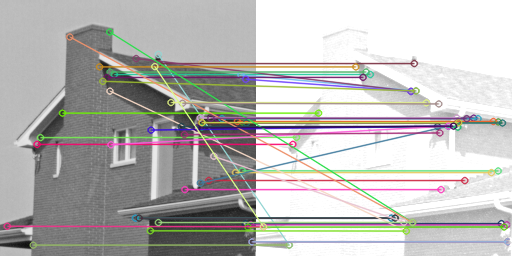
\includegraphics[scale=0.6]{/home/shikhar/Documents/PycharmProjects/Assignment-1/Solution_Report/q2/match1_4.png}
	\caption{Matching with changed illumination }
\end{figure}
\begin{figure}[h]
	\centering
	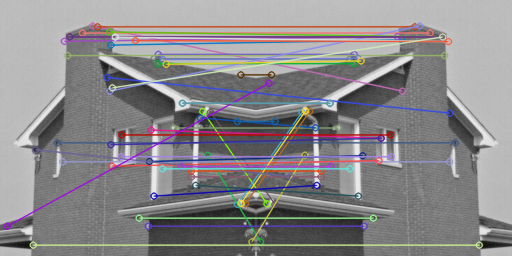
\includegraphics[scale=0.6]{/home/shikhar/Documents/PycharmProjects/Assignment-1/Solution_Report/q2/match1_5.png}
	\caption{Matching with flipped image}
\end{figure}



\end{homeworkProblem}

\clearpage
\begin{homeworkProblem}
\subsection*{Implementation:}
\paragraph{}
For demonstrating object recognition using SIFT algorithm, I took five images from five different categories namely, giraffe, cup, book, cat, and bottle as shown here:

\begin{figure}[ht]
	\centering
	
	\caption*{\textbf{Images used for Object detection}}
	\fbox{\includegraphics[width=2.6cm, height=2.75cm]{/home/shikhar/Documents/PycharmProjects/Assignment-1/Images/q3/giraffe/1.jpg}}
	\fbox{\includegraphics[width=2.6cm, height=2.75cm]{/home/shikhar/Documents/PycharmProjects/Assignment-1/Images/q3/giraffe/2.jpg}}
	\fbox{\includegraphics[width=2.6cm, height=2.75cm]{/home/shikhar/Documents/PycharmProjects/Assignment-1/Images/q3/giraffe/3.jpg}}
	\fbox{\includegraphics[width=2.6cm, height=2.75cm]{/home/shikhar/Documents/PycharmProjects/Assignment-1/Images/q3/giraffe/4.jpg}}
	\fbox{\includegraphics[width=2.6cm, height=2.75cm]{/home/shikhar/Documents/PycharmProjects/Assignment-1/Images/q3/giraffe/5.jpg}} \linebreak \\
	
	\fbox{\includegraphics[width=2.6cm, height=2.75cm]{/home/shikhar/Documents/PycharmProjects/Assignment-1/Images/q3/bottle/1.jpg}}
	\fbox{\includegraphics[width=2.6cm, height=2.75cm]{/home/shikhar/Documents/PycharmProjects/Assignment-1/Images/q3/bottle/2.jpg}}
	\fbox{\includegraphics[width=2.6cm, height=2.75cm]{/home/shikhar/Documents/PycharmProjects/Assignment-1/Images/q3/bottle/3.jpg}}
	\fbox{\includegraphics[width=2.6cm, height=2.75cm]{/home/shikhar/Documents/PycharmProjects/Assignment-1/Images/q3/bottle/4.jpg}}
	\fbox{\includegraphics[width=2.6cm, height=2.75cm]{/home/shikhar/Documents/PycharmProjects/Assignment-1/Images/q3/bottle/5.jpg}} \linebreak \\
	
	\fbox{\includegraphics[width=2.6cm, height=2.75cm]{/home/shikhar/Documents/PycharmProjects/Assignment-1/Images/q3/cat/1.jpg}}
	\fbox{\includegraphics[width=2.6cm, height=2.75cm]{/home/shikhar/Documents/PycharmProjects/Assignment-1/Images/q3/cat/2.jpg}}
	\fbox{\includegraphics[width=2.6cm, height=2.75cm]{/home/shikhar/Documents/PycharmProjects/Assignment-1/Images/q3/cat/3.jpg}}
	\fbox{\includegraphics[width=2.6cm, height=2.75cm]{/home/shikhar/Documents/PycharmProjects/Assignment-1/Images/q3/cat/4.jpg}}
	\fbox{\includegraphics[width=2.6cm, height=2.75cm]{/home/shikhar/Documents/PycharmProjects/Assignment-1/Images/q3/cat/5.jpg}} \linebreak \\
	
	\fbox{\includegraphics[width=2.6cm, height=2.75cm]{/home/shikhar/Documents/PycharmProjects/Assignment-1/Images/q3/book/1.jpg}}
	\fbox{\includegraphics[width=2.6cm, height=2.75cm]{/home/shikhar/Documents/PycharmProjects/Assignment-1/Images/q3/book/2.jpg}}
	\fbox{\includegraphics[width=2.6cm, height=2.75cm]{/home/shikhar/Documents/PycharmProjects/Assignment-1/Images/q3/book/3.jpg}}
	\fbox{\includegraphics[width=2.6cm, height=2.75cm]{/home/shikhar/Documents/PycharmProjects/Assignment-1/Images/q3/book/4.jpg}}
	\fbox{\includegraphics[width=2.6cm, height=2.75cm]{/home/shikhar/Documents/PycharmProjects/Assignment-1/Images/q3/book/5.jpg}} \linebreak \\
	
	\fbox{\includegraphics[width=2.6cm, height=2.75cm]{/home/shikhar/Documents/PycharmProjects/Assignment-1/Images/q3/cup/1.jpg}}
	\fbox{\includegraphics[width=2.6cm, height=2.75cm]{/home/shikhar/Documents/PycharmProjects/Assignment-1/Images/q3/cup/2.jpg}}
	\fbox{\includegraphics[width=2.6cm, height=2.75cm]{/home/shikhar/Documents/PycharmProjects/Assignment-1/Images/q3/cup/3.jpg}}
	\fbox{\includegraphics[width=2.6cm, height=2.75cm]{/home/shikhar/Documents/PycharmProjects/Assignment-1/Images/q3/cup/4.jpg}}
	\fbox{\includegraphics[width=2.6cm, height=2.75cm]{/home/shikhar/Documents/PycharmProjects/Assignment-1/Images/q3/cup/5.jpg}}
	
\end{figure}

\clearpage
\paragraph{Model Transformation}
From all the images the first image from each category was selected as the model image. From each model image, three more images were generated by adding different degrees of noise and flipping the image. As shown here:

\begin{figure}[ht]
	\centering
	\caption*{\textbf{Transformations of a model image}}
	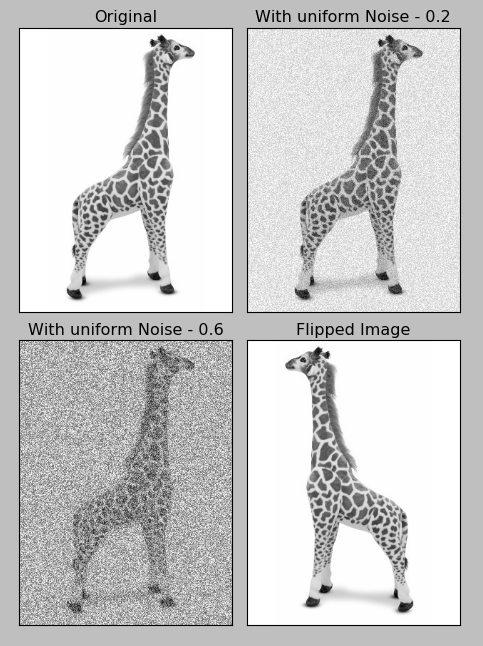
\includegraphics[scale=.5]{/home/shikhar/Documents/PycharmProjects/Assignment-1/Images/q3/trans.png}
\end{figure}

\paragraph{Training classifier}
For training the classifier, descriptors of all the model images and the derieved images were computed using SIFT algorithm and were stored. For predicting category of a new image its descriptors were calculated and were matched with the stored descriptors using k-nearest neighbor approach. Then based on the number of matches the category of the image is predicted. 

\clearpage
\subsection*{Results:}
\paragraph{}
Using the technique mentioned above, the classifier was trained and was used for predicting the category of all the 25 images. The following table shows the performance of the classfier:

\begin{center}
	\begin{tabular}{||c c c c||} 
		\hline
		\textbf{Image index} & \textbf{Actual Category} & \textbf{Predicted Category} & \textbf{Conclusion}\\ [0.5ex] 
		\hline\hline
		(0,0) & Giraffe & Giraffe & \color{ForestGreen}  Correct \\ \hline
		(0,1) & Giraffe & Cup & \color{Red} Incorrect \\ \hline
		(0,2) & Giraffe & Cat & \color{Red} Incorrect \\ \hline
		(0,3) & Giraffe & Cat & \color{Red} Incorrect \\ \hline
		(0,4) & Giraffe & Cup & \color{Red} Incorrect \\ \hline
		(1,0) & Cup & Cup & \color{ForestGreen}  Correct \\ \hline
		(1,1) & Cup & Cup & \color{ForestGreen}  Correct \\ \hline
		(1,2) & Cup & Cup & \color{ForestGreen}  Correct \\ \hline
		(1,3) & Cup & Cup & \color{ForestGreen}  Correct \\ \hline
		(1,4) & Cup & Cup & \color{ForestGreen}  Correct \\ \hline
		(2,0) & Bottle & Bottle & \color{ForestGreen}  Correct \\ \hline
		(2,1) & Bottle & Cup & \color{Red} Incorrect \\ \hline
		(2,2) & Bottle & Book & \color{Red} Incorrect \\ \hline
		(2,3) & Bottle & Cup & \color{Red} Incorrect \\ \hline
		(2,4) & Bottle & Bottle & \color{ForestGreen}  Correct \\ \hline
		(3,0) & Cat & Cat & \color{ForestGreen}  Correct \\ \hline
		(3,1) & Cat & Cat & \color{ForestGreen}  Correct \\ \hline
		(3,2) & Cat & Cat & \color{ForestGreen}  Correct \\ \hline
		(3,3) & Cat & Bottle & \color{Red} Incorrect \\ \hline
		(3,4) & Cat & Cat & \color{ForestGreen}  Correct \\ \hline
		(4,0) & Book & Book & \color{ForestGreen}  Correct \\ \hline
		(4,1) & Book & Book & \color{ForestGreen}  Correct \\ \hline
		(4,2) & Book & Book & \color{ForestGreen}  Correct \\ \hline
		(4,3) & Book & Cup & \color{Red} Incorrect \\ \hline
		(4,4) & Book & Giraffe & \color{Red} Incorrect \\ \hline		
	\end{tabular}
\end{center}

$$\text{\textbf{Average accuracy}} = \frac{\text{Total correct predictions}}{\text{Total number of images}} * 100= \frac{15}{25} * 100= 60\%$$

\paragraph{}
The above result shows the efficiency of SIFT algorithm for finding the right generic descriptors of any given image which can be used to recognize new images of the same type. 

\paragraph{Poor performance on complex inputs}
In above setup all images have white background and the shapes of the images are considerably different but if we take more complex or similar looking images then the algorithm performs poorly. In the given categories if we replace bottles with cycle which are much more complicated images then accuracy falls to 36\%. Moreover, if intead of taking images with white backgroud we take images with background then also accuracy falls considerably. So, although the algorithm is efficient but is not the best choice in all situations.


\end{homeworkProblem}


\end{document}